\subsection{Centralizando los Datos} \label{sec:Centering}

Lo primero para la implementación del observador, era determinar como este tendría acceso al estado de referencia. Hasta el momento, únicamente \textit{Lexical} tiene el contexto definido por el usuario, por lo que era necesario definir una manera mediante la cual otros servicios puedan acceder a este.

Partiendo de la división de responsabilidades, se estableció el implementar un agregador, que contenga el estado definido por el usuario; desde el cual otros servicios puedan acceder a estos datos. 

Esto tiene dos ramificaciones adicionales. La primera, es que abre a la posibilidad de declarar más de una aplicación en simultaneo, usando el agregador como un \textit{hub} que permita guardar y consultar los estados de las aplicaciones que se registren, teniendo una instancia de observador por cada una de ellas.

La segunda, posibilita el usar este agregador para almacenar los estados actuales reportados por el observador. Esto se debe a que, las condiciones para evaluar el estado de las aplicaciones, se encuentran en las propiedades definidas por el usuario durante la declaración del estado de referencia. Siendo así, es posible ver el estado objetivo a partir de las propiedades; y el estado actual basado en la evaluación de los componentes registrados en los requerimientos de datos.

De lo anterior, podemos planear un diagrama, visto en la figura \ref{fig:StarDuckMini}, que refleje el estado actual de la arquitectura del proyecto.

\begin{figure}[ht]
    \centering
    \caption{\\Arquitectura actual del proyecto con el agregador}
    \label{fig:StarDuckMini}
    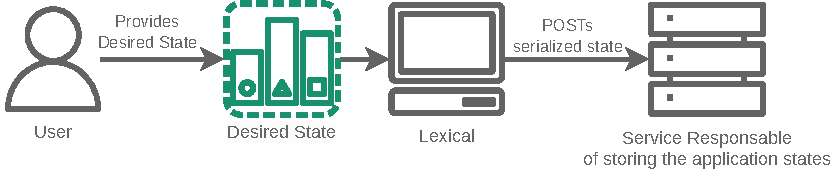
\includegraphics[width=0.9\linewidth]{images/StarDuckMini.pdf}
\end{figure}

La implementación de este agregador, apodado \textit{Bran}\footnote{El código fuente de Bran puede encontrarse en el repositorio \url{https://github.com/ChipDepot/Bran}}, fue relativamente directa. Este tiene dos requerimientos, el primero, es la capacidad de recibir, guardar y actualizar los estados de las aplicaciones; y segundo, el poder enviar los estados almacenados cada vez que estos se soliciten.

Ambas de estas funcionalidades se implementaron usando el framework \texttt{Axum}\footnote{Axum es un framework modular para aplicativos web Open Source desarrollado en Rust. Más información sobre este puede encontrarse en su repositorio \url{https://github.com/tokio-rs/axum}}. Usando como base la librería \textit{StarDuck}, se definió un único endpoint que toma, \texttt{apps/:app\_name}, que acepta peticiones de tipo \texttt{GET}, para consultar el estado de la aplicación; \texttt{POST} y \texttt{PUT}, para el registro inicial de la aplicación, y posterior actualización de esta. 

Ya con el servicio implementado se agregó, a \textit{Lexical}, un cliente HTTP con el cual, tras validar la arquitectura objetivo proveída por el usuario, y como se ve en la figura \ref{fig:StarDuckMini}, este realice una petición de tipo POST a la una instancia de \textit{Bran} indicada con el fin de registrarla. Una versión actualizada del proceso realizado \textit{Lexical} puede verse en la figura \ref{fig:UpdatedLexicalFlow}.

\begin{figure}[ht]
    \centering
    \caption{\\Diagrama de flujo del proceso realizado por Lexical actualizado}
    \label{fig:UpdatedLexicalFlow}
    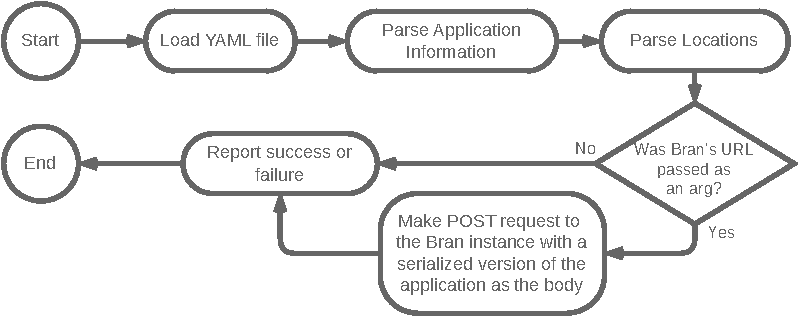
\includegraphics[width=0.9\linewidth]{images/UpdatedLexicalFlow.pdf}
\end{figure}